\documentclass[border=3pt,tikz]{standalone}

\usepackage{mathtools}
\usetikzlibrary{decorations.markings}

\colorlet{Ecolor}{orange!90!black}
\colorlet{pluscolor}{red!60!black}
\colorlet{minuscolor}{blue!60!black}
\tikzstyle{anode}=[top color=red!20, bottom color=red!50]
\tikzstyle{cathode}=[top color=blue!20, bottom color=blue!40]
\tikzstyle{charge+}=[very thin,top color=red!50, bottom color=red!80]
\tikzstyle{charge-}=[very thin,top color=blue!40, bottom color=blue!70]
\tikzset{EFieldLine/.style={
  Ecolor, decoration={markings, mark=at position #1 with {\arrow{stealth}}}, postaction={decorate}}
}

\def\dph{0.3} % dipole height
\def\dpw{0.1} % dipole width
\def\dipole#1{
  \begin{scope}[shift={(#1)}]
    \draw[charge-] (-\dph,0) to[out=90,in=180] (0,\dpw) -- (0,-\dpw) to[out=180,in=-90] cycle;
    \draw[charge+] ( \dph,0) to[out=90,in=0] (0,\dpw) -- (0,-\dpw) to[out=  0,in=-90] cycle;
    \node[scale=0.7] at (-\dph/2,0) {$-$};
    \node[scale=0.7] at ( \dph/2,0) {$+$};
  \end{scope}
}

\def\height{5}
\def\width{3}
\def\platewidth{0.5}
\def\dielwidth{0.13*\width}
\def\nfieldlines{6}
\def\ncharges{7}

\begin{document}
% capacitor with dipolar polarization
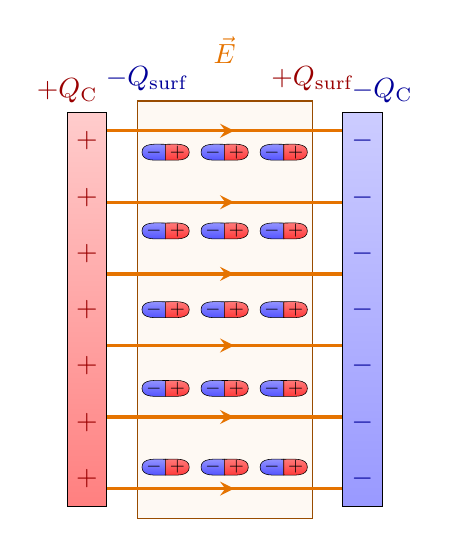
\begin{tikzpicture}

  % dielectric slab
  \draw[orange!60!black,fill=orange!80!brown!5]
  (\dielwidth,-0.03*\height) rectangle (\width-\dielwidth,1.03*\height)
  node[Ecolor, above=3cm, midway] {$\vec E$}
  node[above, pluscolor] {$+Q_\text{surf}$}
  node[above, minuscolor] at (1.3*\dielwidth,1.03*\height) {$-Q_\text{surf}$};

  % electric field
  \foreach \i [evaluate={\y=(\i-0.75)*\height/(\nfieldlines-0.5);}] in {1,...,\nfieldlines}{
      \draw[EFieldLine={0.54},very thick] (0,\y) --++ (\width,0);
    }

  % plates
  \draw[anode] (0,0) rectangle++ (-\platewidth,\height)
  node[above, pluscolor] {$+Q_\text{C}$};
  \draw[cathode] (\width,0) rectangle++ (\platewidth,\height)
  node[above, minuscolor] {$-Q_\text{C}$};

  \foreach \i [evaluate={\y=(\i-0.5)*\height/\ncharges;}] in {1,...,\ncharges}{
      \node[pluscolor] at (-\platewidth/2,\y) {$+$};
      \node[minuscolor] at (\width+\platewidth/2,\y) {$-$};
    }

  % dipoles
  \foreach \i in {0.25, 0.5, 0.75}{
      \foreach \j in {1, 3, 5, 7, 9}{
          \dipole{\i*\width,0.\j*\height}
        }
    }

\end{tikzpicture}
\end{document}
